\documentclass[12pt,a4paper]{article}
\usepackage{comment}
\usepackage[hidelinks]{hyperref}
\usepackage{listings}
\usepackage{graphicx}
\usepackage{subcaption}
\usepackage{float}
\usepackage[table,xcdraw]{xcolor}

\begin{comment}
    https://www.tablesgenerator.com/#
    We can create tables with this page so its easier to portray our examples
\end{comment}

\title{%
    \vspace*{-5mm}\Huge GW2-SRS TRANSFORM \\
    \vspace*{2mm}\Large powered by \LaTeX}

\author{\vspace*{-5mm}\large Daniel Lopez: \textbf{Transform algorithm}}

\begin{document}

    \maketitle

    \begin{figure}[H]
        \centering
        
\includegraphics[width=1 \textwidth]{Images/Nuevo_logo_GW2.png}
    \end{figure}

    \newpage

    \section*{2.0 TRANSFORM}

    \section*{\large 2.1 Introduction}
    After completing the data extraction, it was needed to do a deep cleaning on the files.
    The extracted data was displayed on the HTML source as a JSON type, it as well contained
    lots of information that is entirely related to the statistics in-game. Whether is true that
    statistics showed player names, player accounts, DPS\footnote{Damage Per Second}, etc. It
    also showed information that wasn't needed at all, where we could find EliteInsights information
    about it's version, release and EVTC\footnote{Unique log filetype from ArcDPS app} version as well.\\

    Therefore, I only wanted to gather clear stats data that could help me in the further
    analysis. The data I decided to aim for was:
    \begin{itemize}
        \item Player name
        \item Player Account
        \item Player Profession/Class
        \item Player DPS Statistics
    \end{itemize}

    \begin{table}[!h]
        \begin{tabular}{|c|llll}
        \hline
                                           & \multicolumn{1}{c|}{\cellcolor[HTML]{CBCEFB}Player's Name} & \multicolumn{1}{c|}{\cellcolor[HTML]{CBCEFB}Player's Account} & \multicolumn{1}{c|}{\cellcolor[HTML]{CBCEFB}Player's Class} & \multicolumn{1}{c|}{\cellcolor[HTML]{CBCEFB}Player's DPS} \\ \hline
        \cellcolor[HTML]{FFCCC9}\textbf{1} & \multicolumn{1}{c}{John\_Doe}                              & \multicolumn{1}{c}{johndoe.9752}                              & \multicolumn{1}{c}{Catalyst}                                & \multicolumn{1}{c}{35867.43}                              \\ \cline{1-1}
        \cellcolor[HTML]{FFCCC9}\textbf{2} & ...                                                        &                                                               &                                                             &                                                           \\ \cline{1-1}
        \cellcolor[HTML]{FFCCC9}\textbf{3} &                                                            &                                                               &                                                             &                                                           \\ \cline{1-1}
        \end{tabular}
    \end{table}

    \newpage

    \section*{\large 2.2 In-depth data explanation}

    \subsection*{\normalsize 2.2.1 JSON format}
    In order to understand the data, I had to read and investigate the JSON files lots of times.
    Due to the JSON files size, I decided to use a JSON Viewer\footnote{http://jsonviewer.stack.hu/} 
    to help me with this task.\\

    \begin{figure}[h!]
        \centering
        \begin{subfigure}[b]{0.8\linewidth}
          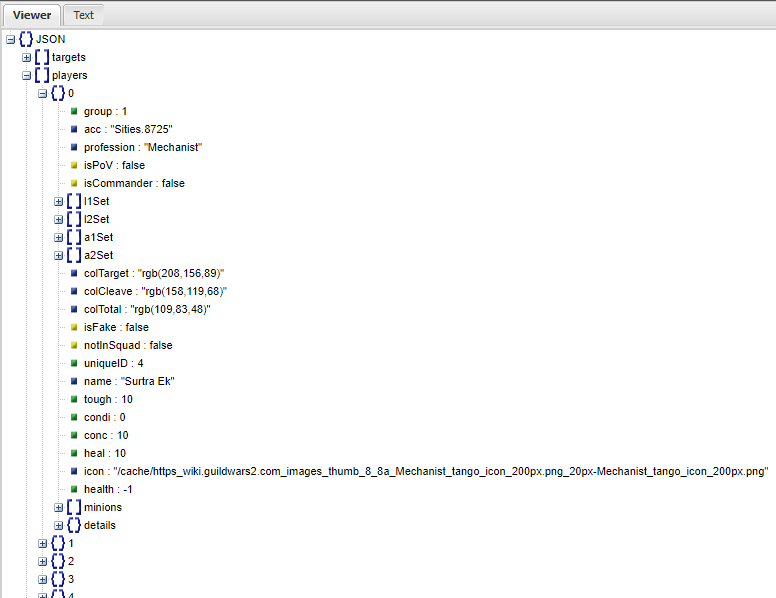
\includegraphics[width=\linewidth]{Images/json_schema.png}
          \caption{JSON Viewer formatted schema}
        \end{subfigure}

        \begin{subfigure}[b]{0.8\linewidth}
          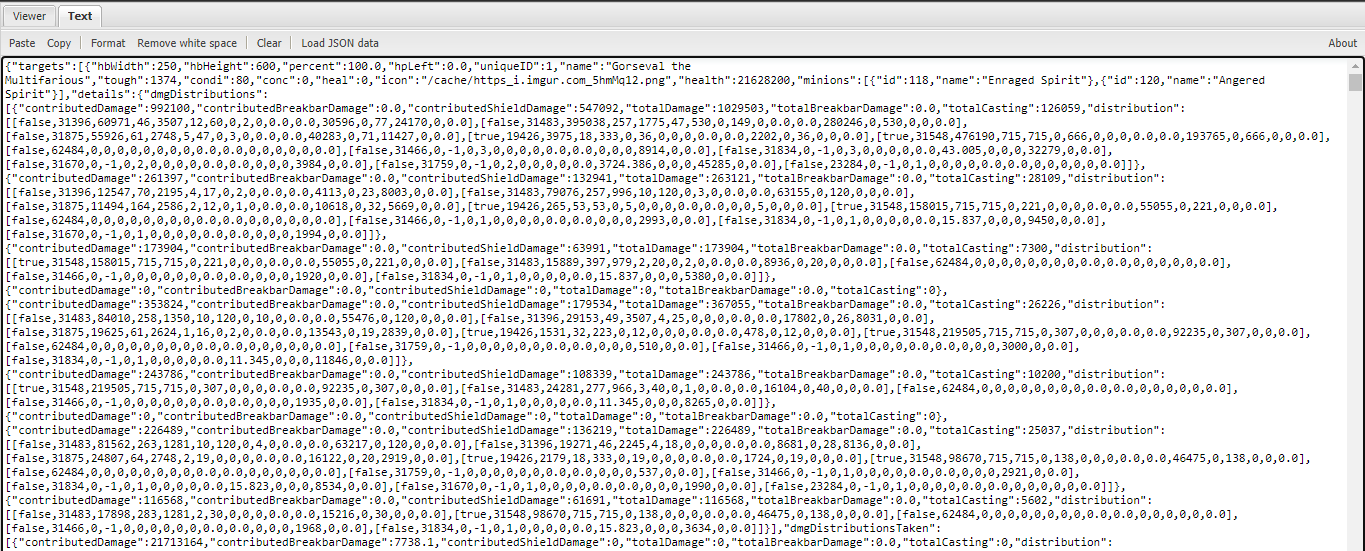
\includegraphics[width=\linewidth]{Images/json_raw.png}
          \caption{Raw JSON view}
        \end{subfigure}
    \end{figure}

    \newpage

    Using this method made the search of information extremely easy, for the most part, the essential
    player data like names, accounts and professions was pretty much finding each player and this data
    by it's index. I applied a zipped For loop to do the aggregation on SQL databases and on No-SQL databases
    I used a simple dictionary I created and then passed as a JSON dictionary.\\

    \begin{lstlisting}[language=Python, caption={\textbf{Basic player data loop}},captionpos=!b]
        for player in data['players']:
            player_group.append(player['group'])
            player_acc.append(player['acc'])
            player_names.append(player['name'])
            player_classes.append(player['profession'])
    \end{lstlisting}
    \begin{lstlisting}[language=Python, caption={\textbf{Custom Python stat dictionary}},captionpos=!b]
        stats_dict = {
                'boss': target,
                'players':{
                    'group': player_group,
                    'account': player_acc,
                    'names': player_names,
                    'profession': player_classes,
                    'phase_1_dps': player_dps1,
                    'phase_2_dps': player_dps2,
                    'phase_3_dps': player_dps3
                }
            }
    \end{lstlisting}
    
    \begin{lstlisting}[language=Python, caption={\textbf{Zipped data for SQLite query}},captionpos=!b]
        for (name,acc,profession) in zip \
        (player_names,player_acc,player_classes):
    \end{lstlisting}

    It was important using a zipped For loop since the query need to be executed for every player.
    This is indeed not efficient if we look into the repetition of the same query for a simple operation
    but since there are only 10 players per boss fight, it ended up being rather useful.

    \newpage

    \subsection*{\normalsize 2.2.2 DPS data}
    Finding each boss DPS data was indeed a quite difficult task. In order to get deeper in this topic
    I must explain a few concepts from Guild Wars 2 game itself.

    Guild Wars 2 is an MMO having different classes or profession that the player can create, however, in
    raid, strikes and fractals, we must have in mind that classes have two kind of damage: Condition damage
    and Power damage. This is important to understand since the DPS on each boss, and for each player, is divided
    between Condition and Power as well as it has a combination of both.

    Every class in the game can deal both Power and Condition, but some classes are more suitable to deal Power
    damage and some other classes are more suitable to deal Condition damage.

    Once explained this, we can get a bit deeper into the data. As I said before, the DPS data has three values
    per phase:
    \begin{itemize}
        \item Power + Condition
        \item Condition
        \item Power
    \end{itemize} 

    There are more data stored in the JSON, but what I needed is essentially this. I used the combined one, and
    you may wonder why not use the specific damage for each class. This not only would be extremely inefficient in
    the long run, but also, damage is also affected but extra aspects and boons added by other classes, so even if
    you are a Power class, you could get a buff from a Thief class making your attacks deal Poison damage which is 
    considered a Condition. Therefore, using the combined one is rather a better option.

    \newpage

    Another important fact to now is that, each boss has different phases. It's true that some bosses share same phases
    and same index, but this does not represent the majority of the bosses. Therefore, each boss needs its own index
    founder. It looks like this in the actual code:

    \begin{lstlisting}[language=Python]
    if nameTag == 'vg':

            # Phase_1
            phase1 = data['phases'][1]['dpsStats']

            phase1_time_raw = data['phases'][1]['duration']
            phase1_time = round(phase1_time_raw/1000,1)

            for dps in phase1:
                dps1_raw = dps[0]
                player_dps1.append(round(dps1_raw/phase1_time,2))

            # Phase_2
            phase2 = data['phases'][6]['dpsStats']

            phase2_time_raw = data['phases'][6]['duration']
            phase2_time = round(phase2_time_raw/1000,1)

            for dps in phase2:
                dps2_raw = dps[0]
                player_dps2.append(round(dps2_raw/phase2_time,2))

            # Phase_3
            phase3 = data['phases'][12]['dpsStats']

            phase3_time_raw = data['phases'][12]['duration']
            phase3_time = round(phase3_time_raw/1000,1)

            for dps in phase3:
                dps3_raw = dps[0]
                player_dps3.append(round(dps3_raw/phase3_time,2))
    \end{lstlisting}

    \newpage

    We are applying several things here. For instance, every boss has between 3 and 6 phases where you can actually damage it,
    this doesn't mean that there are no extra phases, but the damage there is really not that important or substantial to have
    it in mind for an analysis. Therefore, I picked the main phases and made a set of operations over it:

    \begin{itemize}
        \item I applied a For loop on every phase, so it saves the damage dealt for every player.
        \item This information is appended to an empty list.
        \item Finally, but really important, all the damage is divided by the time phase.
    \end{itemize}

    \bigskip

    If we look at the JSON file, it's easy to see that all phase timestamps are written like a single int number (i.e: 190s = 190000),
    this was actually problematic when trying to divide the phase dmg numbers. So the best option I found to deal with this problem
    was dividing it by 1000 so it shows time in seconds and therefore division could be executed better. To end with this data, I just
    applied a \textbf{round} operation.

    \begin{figure}[b]
        \centering
        \begin{subfigure}[b]{0.15\linewidth}
            \href{https://github.com/icharo-tb}{
\includegraphics[width=\linewidth]{Images/GitHub-logo.png}}
        \end{subfigure}
        \begin{subfigure}[b]{0.15\linewidth}
            \href{https://www.linkedin.com/in/danielopezpajares/}{
\includegraphics[width=\linewidth]{Images/LinkedIn_Logo.png}}
        \end{subfigure}
        \begin{subfigure}[b]{0.15\linewidth}
            \href{https://gitlab.com/daniel.lopez.pajares.2021}{
\includegraphics[width=\linewidth]{Images/GitLab_logo.png}}
        \end{subfigure}
    \end{figure}
\end{document}